\documentclass{article}
\usepackage[utf8]{inputenc}
%\usepackage{biblatex}
\usepackage{amssymb}
\usepackage{amsmath}
\usepackage{amsthm}
\usepackage{graphicx}
\usepackage{float}
\usepackage{url}
\usepackage{framed}
\usepackage{booktabs}
\usepackage{enumitem}
\usepackage{extarrows}
\usepackage{subcaption}
\usepackage{epstopdf}
\usepackage{hyperref}
%\usepackage{algorithm}
%\usepackage{algorithmic}
\usepackage[ruled,linesnumbered]{algorithm2e}
\numberwithin{equation}{section}
%\usepackage{BOONDOX-calo}
\title{Research Proposal: Partially coherent ptychography}
%\author{huibinchang }
\date{July 2021}

\begin{document}

\maketitle
\tableofcontents
\section{Introduction}

%Please describe your proposed research topic (up to 500 characters including spaces).
%The description should include the general field of the research and the specific research question(s).

Ptychography is a popular imaging technique in scientific fields as diverse as condensed matter physics, cell biology, materials science, and electronics, among others. In a coherent Ptychography experiment, a localized coherent X-ray probe (or illumination) scans through a specimen, while the detector collects a sequence of phaseless intensities in the far-field. The goal is to obtain a high-resolution reconstruction of the specimen from the sequence of intensity measurements. 

Coherent Ptychographic imaging experiments often rely on apertures to define a coherent illumination. Research institutions around the world are investing considerable resources to produce brighter x-ray sources to overcome this limitation. Meanwhile, most of the x-ray photons generated are currently discarded by secondary apertures. Even when there is enough coherent flux, the stability required during exposure is often another limiting factor. In a word, coherent light sources need strict experiment conditions and could cause waste. Both flux and stability limitations can be reduced using partial coherence analysis. 


%Ptychography is a popular imaging technique in scientific fields like condensed matter physics, cell biology, materials science, and electronics, etc. Its goal is to obtain a high-resolution reconstruction of the specimen from the sequence of intensity measurements. Traditional Ptychographic imaging experiments often rely on apertures to define a coherent illumination, which is strict and could cause waste. Both flux and stability limitations can be reduced using partial coherence analysis. 

\section{Objectives}

Generally speaking, we would like to characterize partially coherent to Mathematical language and design an effective algorithm to solve the problem. To prove the rationale of the model and algorithm, quantitative analysis is required to characterize the approximation error of the model and the convergence speed of the algorithm, under suitable assumptions for the phobe and the vibration kernel for a partially coherent effect.





\section{Methods}
\begin{enumerate}[leftmargin=*]
\item Model

Models would be borrowed from physics literature and transformed into mathematical language. Because various models are used to characterize partially coherent effects in different settings, we would like to build connections between models through applied analysis skills. To obtain a high-resolution reconstruction of the specimen from the sequence of intensity measurements, we need to solve an inverse problem, which would be described as an optimization problem. 

\item Algorithm 

There are plenty of optimization algorithms available, like the Gradient descent method.
Considering the non-convex and low-rank nature of this problem, we would focus on algorithms in these fields \cite{lowrank}\cite{ADMM}, and make innovative adjustments utilizing the structure inside the specific model.

\item Experiment

The algorithm would first be tested on simulation data. Then, we would get data from SLAC National Accelerator Laboratory and test on real-world data.

\item Convergence Analysis

For non-convex optimization, we could follow the general framework in \cite{nonconvex}.



\end{enumerate}

\section{Background/prior work}

\begin{enumerate}[leftmargin=*]

\item Model 

We would mainly investigate three models. \cite{mix} proposes a general model based on quantum state tomography. The phobe is assumed to be in a mixed state to represent a partially coherent effect.
\begin{equation}
\label{sep} 
\begin{aligned}
&\mbox{Find } u, r \mbox{ othogonal $w_k$   }s.t. \\
&f_{p c, j}=\sum_{k=1}^r \left|\mathcal{F}\left( \mathcal{S}_{j} u \circ \left(\omega_k\right) \right)\right|^{2} (0\leq j \leq N-1)
\end{aligned}
\end{equation}
Another form:
\begin{equation}
\label{lift}
\begin{aligned}
&\mbox{Find } u,\rho,s.t.\\
&f_{pc,j}(q) = Tr(\mathcal{I}_{j \mathbf{q}} \rho ) (0\leq j \leq N-1)\\
&\rho \mbox{ is positive semi-definite, with rank}\leq r 
\end{aligned}
\end{equation}

 \cite{psf} and vibration model \cite{chang} are two specific ones:
 
 \begin{equation}
 \label{simple}
     f_{p c}=f * \kappa
 \end{equation}
 
 \begin{equation}
 f_{p c, j}=\sum_{i} \kappa_{i}\left|\mathcal{F}\left( \mathcal{S}_{j} u \circ \left(\mathcal{T}_{i} \omega\right) \right)\right|^{2}
 \label{model:target}
 \end{equation}
 

We have shown that \ref{model:target} in a special case of \ref{sep}. Though numerical experiment shows that the density matrix $\rho$ in vibration model is approximated low-rank, no theoretical analysis has been conducted, and the suitable number of states remains empirical. Besides, the decomposed modes are amazingly beautiful, some of which are similar to derivations of the main mode. We used Functional expansion skills like Taylor expansion to expand the phobe under some smooth conditions and got primary explanations.  


\begin{figure}[H]
\centering

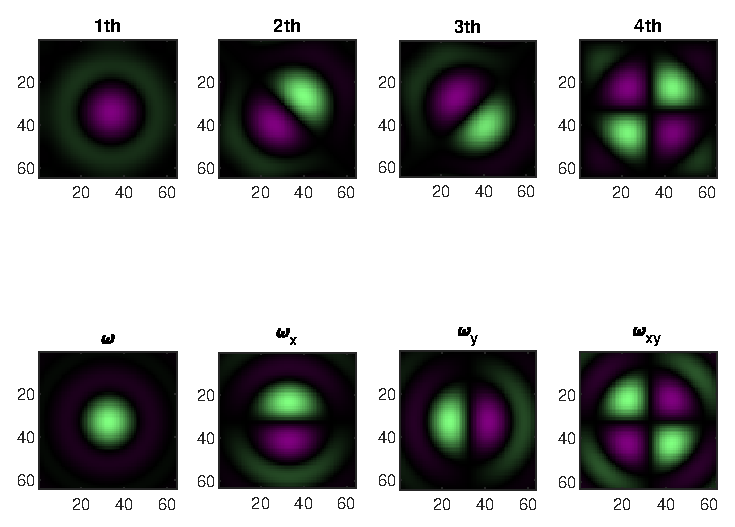
\includegraphics[width=0.9\linewidth]{../figures/gradients.eps} 
\caption{Decomposed modes} 
 \end{figure}
 
 \begin{figure}[H]
  \begin{subfigure}{.5\textwidth}
    \centering
    % include first image
    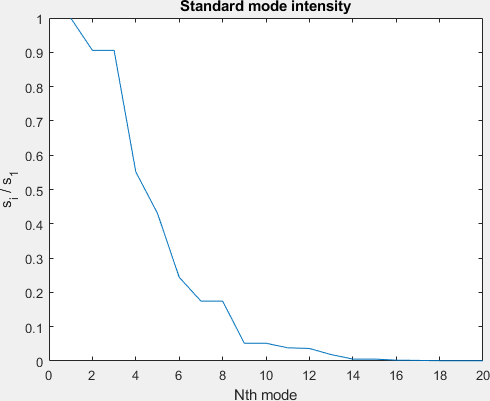
\includegraphics[width=0.9\linewidth]{../figures/singular.png}  
    %\caption{}
    \label{fig:singular}
  \end{subfigure}
  \begin{subfigure}{.5\textwidth}
    \centering
    % include second image
    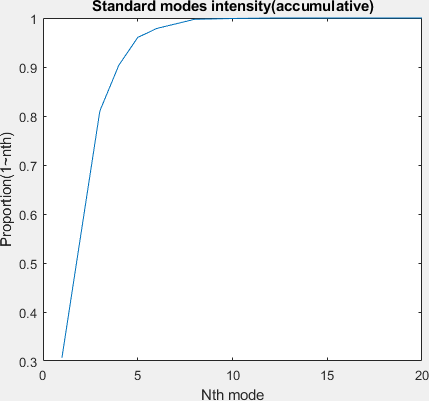
\includegraphics[width=.8\linewidth]{../figures/singular_accumative.png}  
    %\caption{Put your sub-caption here}
    \label{fig:singular_acc}
  \end{subfigure}
  \caption{The distribution of singular values of the standard density matrix $\rho$. The vertical axis in the left subfigure represents the ratio of $i^{th}$ largest singular to the first one $s_i/s_1$, and that in the right one represents $S_{cum}(i)$. The singular value decreases exponentially and the matrix is approximately low-rank. }
  \label{fig:standard singular}
  \end{figure}
  
 
  

\item Problem solving

 ADMM algorithm has been used to solve coherent Ptychography problem with convergence analysis\cite{admm}. In a partially coherent problem, an intuitive AP(alternative projection) algorithm was commonly used. We firstly extended the ADMM algorithm to mixed states, and then tried adjustments to supplement the searching process, like adding orthogonal constraints.
 
\item Experiment

 We used a general model and extended ADMM algorithm, conducting Experiments similar to \cite{chang}. Our methods could overcome larger partially coherent effects, and experiment results show greater speed over AP.
 
 \begin{figure}[H]
 \centering
 \caption{}
 \begin{subfigure}{1\textwidth}
     \centering
     % include first image
     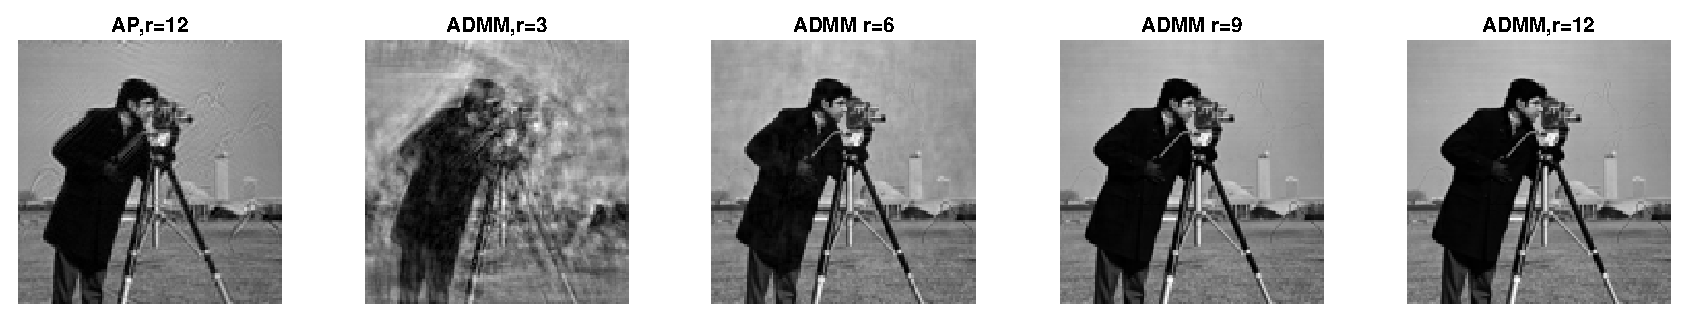
\includegraphics[width=0.9\linewidth]{../figures/modes_u.eps}  
    \caption{Amplitude}
     \label{fig:modes_u}
  \end{subfigure}
  \begin{subfigure}{1\textwidth}
     \centering
     % include second image
     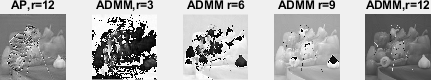
\includegraphics[width=.9\linewidth]{../figures/modes_u_phaze.png}  
     %\caption{Put your sub-caption here}
     \caption{Phase}
     \label{fig:modes_u_phaze}
  \end{subfigure}
  
     \label{fig:modes_images}
 
  \end{figure}
  
  \begin{figure}[H]
  \begin{subfigure}{.5\textwidth}
     \centering
     % include first image
     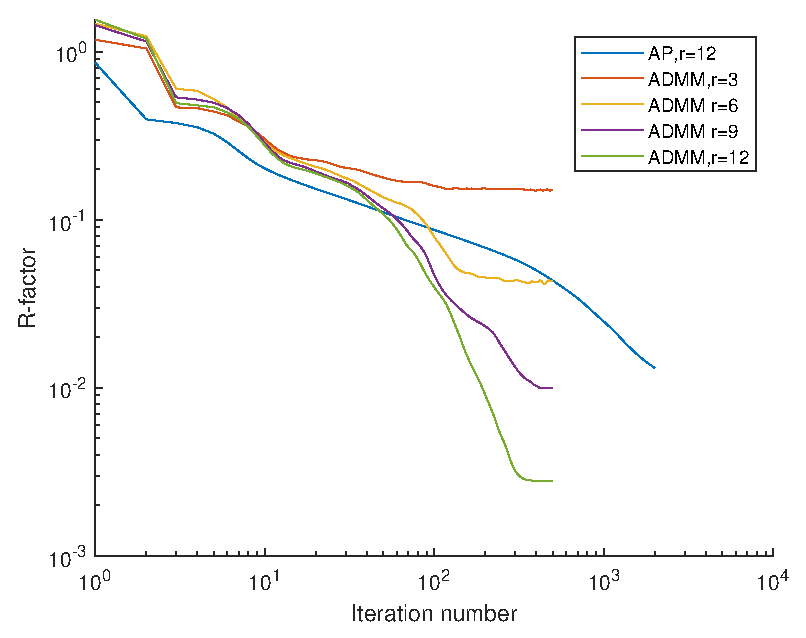
\includegraphics[width=0.9\linewidth]{../figures/modes_R.eps}  
     %\caption{}
     \label{fig:modes_R}
  \end{subfigure}
  \begin{subfigure}{.5\textwidth}
     \centering
     % include second image
     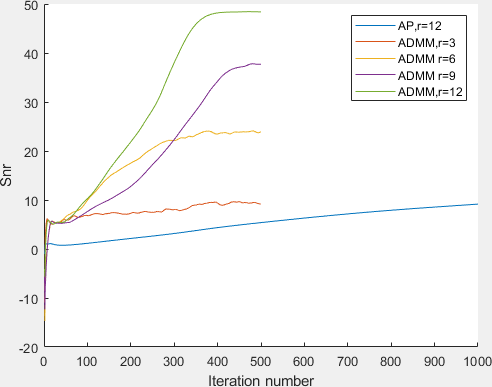
\includegraphics[width=.9\linewidth]{../figures/modes_snr.png}  
     %\caption{Put your sub-caption here}
     \label{fig:modes_snr}
  \end{subfigure}
  \caption{R and snr. }
  \label{fig:noise}
  \end{figure}



\end{enumerate}

\begin{thebibliography}{99}
\bibitem{chang}{Chang, Huibin, et al. "Partially coherent ptychography by gradient decomposition of the probe." Acta Crystallographica Section A: Foundations and Advances 74.3 (2018): 157-169.}
\bibitem{theory}{Wolf E. New theory of partial coherence in the space-frequency domain. Part I: spectra and cross spectra of steady-state sources[J]. JOSA, 1982, 72(3): 343-351.}
\bibitem{mix}{Thibault P, Menzel A. Reconstructing state mixtures from diffraction measurements[J]. Nature, 2013, 494(7435): 68-71.}
\bibitem{direct}{Multiplexed coded illumination for Fourier Ptychography with an LED array microscope.}
\bibitem{algorithm}{Thibault P, Dierolf M, Bunk O, et al. Probe retrieval in ptychographic coherent diffractive imaging[J]. Ultramicroscopy, 2009, 109(4): 338-343.}
\bibitem{quan}{Introduction to Quantum Mechanics, David J. Griffiths, 12.3}
\bibitem{all}{Fannjiang A, Strohmer T. The numerics of phase retrieval[J]. Acta Numerica, 2020, 29: 125-228.}
\bibitem{admm}{Chang, Huibin, Pablo Enfedaque, and Stefano Marchesini. "Blind ptychographic phase retrieval via convergent alternating direction method of multipliers." SIAM Journal on Imaging Sciences 12.1 (2019): 153-185.}
\bibitem{psf}{Konijnenberg S. An introduction to the theory of ptychographic phase retrieval methods[J]. Advanced Optical Technologies, 2017, 6(6): 423-438.}

\bibitem{nonconvex}{Attouch H, Bolte J, Redont P, et al. Proximal alternating minimization and projection methods for nonconvex problems: An approach based on the Kurdyka-Łojasiewicz inequality[J]. Mathematics of operations research, 2010, 35(2): 438-457.}

\bibitem{lowrank}{Candes E J, Strohmer T, Voroninski V. Phaselift: Exact and stable signal recovery from magnitude measurements via convex programming[J]. Communications on Pure and Applied Mathematics, 2013, 66(8): 1241-1274.}

\bibitem{ADMM}{Boyd S, Parikh N, Chu E. Distributed optimization and statistical learning via the alternating direction method of multipliers[M]. Now Publishers Inc, 2011.}



\end{thebibliography}


Tong has a convincing reason of her research interest -- computational and applied mathematics, especially in digital signal
and image processing, and their applications in medicine and neuroscience. First, it is what she is good at and loves. She learned to implement data structures and algorithms in C++ from the first grade of junior high school and got a solid computing foundation through six years of training in programming and algorithm. She participated in the National Youth Computer Competition on behalf of her
senior middle school and won the first prize of the National Olympiad in Informatics in Provinces. She showed even stronger interest in Mathematics - in her words, she is obsessed with the abstraction and
simplicity of mathematical language. 

Moreover, the predicament encountered by her family gave her an extraordinary enthusiasm and interest in solving medical problems with mathematical tools. We are sorry to know that she lost her father because of brainstem hemorrhage, and her mother-in law was admitted to the hospital because of schizophrenia in 2020. She took the responsibility to take care her mother-in law and finished a series of work like recording each prescription, observing her abnormal reactions after the medication, and communication with
the doctor. We could see her optimism and strong heart, and a sensitivity in medical problems. She is eager to solve specific problems like investigating the mechanism of mental illness. We believed that her research would be conducive to understanding how to make full
use of medical data (physiological electrical signals, medical images), develop new medical devices, and
contribute to human health.

To fulfill her goal, she is active to conduct research in computational and applied mathematics. She participated in project ' Registration and 3D reconstruction of serial tissue sections' in cooperation with Sun Yat-sen University Cancer Center from 2021. Her supervisor, Prof. Li Jia in Sun yat-sen University, recognized she made major contribution and largely promoted this project. Besides, she participated in Contemporary Undergraduate Mathematical Contest in Modeling in 2019 and did a followed-up study on 'Data Analysis on the Fairness of Short-trip Taxi Services in Guangzhou Baiyun International Airport'. As a co-first author, Her work is published in the Competition Forum column in Mathematical Modeling and Its Applications, which is a Chinese Journal focusing on mathematical modeling competitions. She showed strong ability in literature search and organization, building models and programming.

In her research plan on Partially coherent Ptychography, she clearly convey the background, objectives, methods, and prior work. Ptychography is a popular imaging technique in scientific fields like condensed matter physics, cell biology,
materials science, and electronics, etc. Partial coherence analysis could benefit high-resolution reconstruction of the specimen
from the sequence of intensity measurements under broad experiment condition.




 





\end{document}